\section{Experiments}
\label{sec:experiments}

\subsection{Data Sets}


We use 5 \href{http://archive.ics.uci.edu/ml/datasets.html}{UCI classification
datasets}:, described as in Table ~\ref{tb:datasets}.

\begin{table}

\begin{tabular}{| c | c |  c | c | c |}
  \hline
  Datasets & \# instances & \# features & class-wise split & sparse\\
  \hline
  Farms Ads dataset & 4,143 & 54,877 & $53.3\%$ vs. $46.7\%$ & yes\\
  \hline
  Amazon Commerce reviews dataset & 1,500 & 10,000 & $50\%$ vs. $50\%$ & yes \\
  \hline
  p53 Mutants dataset & 31420 & 5,409 & $99.52\%$ vs.$0.48\%$  & no\\
  \hline
  Human Activity Recognition dataset & 7352 & 561 & $53.3\%$ vs. $46.7\%$  & no\\
  \hline
  URL Reputation dataset\footnotemark[1] & 16000 & 74113 & $62.7\%$ vs. $37.3\%$ & yes \\
  \hline
\end{tabular}
\caption{Datasets information}
\label{tb:datasets}
\end{table}

The Farm Ads dataset was collected from text ads found on 12 websites that deal with various farm animal related topics. For each ad, features include the words on the ad creative and the words the landing page. Words in creative page are diffirentiated from words from ad landing page by prefixing them with "ad-". Binary labels were manually added to represent if the ad is appropriate for that website. The Amazon Commerce reviews dataset were collected from the customer reviews in Amazon Commerce website for authorship identification. Features of a review consists of text tokens contained in that review. Labels represent the authors of the reviews. The dataset consists of reviews from 50 authors, and 30 reviews per author. The p53 Mutants dataset include features from the biophysical models of mutant p53 proteins, and binary labels represent the p53 transcriptional activity (active or inactive). The Human Activity Recognition dataset was collected from experiments carried out with a group of 30 volunteers. Features include acceleration and angular velocity collected from 3 axes at constant frequency within a fixed length of time. Labels represent the six activities that the subjects can perform. The features of URL Reputation dataset include features collected for each URL, including text tokens in the URL, WHOIS information, location, connection speed and so on. Labels represent if the URL is legal. We preprocessed the datasets to evenly split multi-class datasets (Amazon Commerce reviews and Human Activity Recognition datasets) into two classes.



\footnotetext[1]{The dataset is too large so we used only one day of data out of total 121 days in the dataset.}

\subsection{Results}

\subsubsection{MCMC based estimation}
Our MCMC sampling strategy that we described in section~\ref{sec:MCMCmethod}
converges. Figure~\ref{fig:MCMCconverge} is a plot of the iterations of the Markov 
chain for estimation on a subset of Farms Ads dataset. This is for MLE
estimation without any priors. We also 

\begin{figure}![htb]
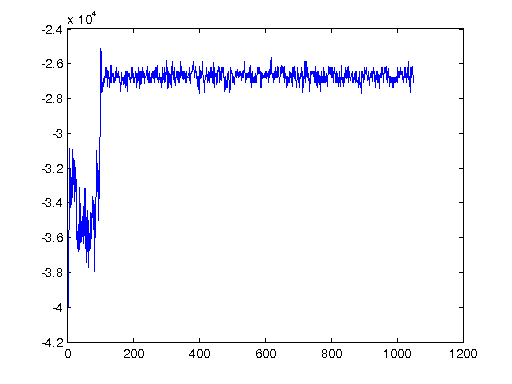
\includegraphics[width=1\textwidth]{samplingConvergence.png}
\caption{Markov chain convergence on Farms ads data. We take a sub-sample of
the dataset: 2000 rows and 100 columns}
\label{fig:MCMCconverge}
\end{figure}